\documentclass[a4paper, % papirstørrelse, skal altid med
final,% Når man skal skifte kompileringsmetode mellem draft og final skal man 
      %flytte kommenteringen %  i Draft kommanoerne, nedenfor.
11pt, % standardstørrelse på fonten
openany%, % anvnedes hvis kapitler bare skal starte på den næste side
%oneside,
%article
]{memoir}%
% marginer, memoir to to metoder
% den traditionelle, se memoir manualen
% venstre: 2.5cm, højre: 3.5cm, top: 3cm, bund: 4cm
%her kan margenen sættes manuelt, hvis man har lyst
%\setlrmarginsandblock{3.5cm}{3.5cm}{*}
%\setlrmarginsandblock{1.5cm}{6.5cm}{*}
%her kan margenen sættes manuelt, hvis man har lyst
%\setulmarginsandblock{3cm}{4cm}{*}
% % mere utraditionelt, men hurtigt smartere
% % vi sætter tekstblokken og placerer den
% % værdierne som er angivet svarer ca. til dem anvende i LaTeXbogen
% % 400pt bred og en højde svarende til at forholdet er det gyldne snit
%\settypeblocksize{*}{300pt}{1.618}
% % placer tekstblokken på papriet, kun en værdi skal angives, her sider
% % vi bare hvad forholder mellem marginerne skal være
% \setlrmargins{*}{*}{1.6}
% \setulmargins{*}{*}{1.3}
\checkandfixthelayout % laver forskellige beregninger og sætter de
% almindelige længder op
\usepackage[utf8]{inputenc} % eller utf8 eller ansinew eller ...
\usepackage[danish]{babel} %direktiv til at bruge det danske sprog

\usepackage[draft]{fixme} % til at skrive \fixme kommentarer til sig

%\newenvironment{Draft}{\fixme{HUSK at ændre kommenteringen i preamble når man skifter mellem draft og final} }{  }
\let\Draft=\comment \let\endDraft=\endcomment


%har vi ord der bliver delt forkert kan de indsættes i hyphernation med bindestreg alle steder hvor ordet kan deles
\hyphenation{tit-len mo-del-len pro-du-ce-rer an-svars-hav-ende om-for-deles for-bind-elses-mulig-heder ska-ber æn-dring-er net-værks-en-hed-er peer backup backup-system fast-track backup-systemer nabo-peers frame-work efter-som Grund-lag-et plads-effek-tivi-teten audits}


\usepackage{nameref}
\usepackage[danish]{varioref} % smarte krydsreferencer via \vref
\usepackage[colorlinks, linkcolor=blue, citecolor=blue, urlcolor=blue, 
final=true]{hyperref}

%giver mulighed for at hoppe i pdf'filen via referencerne.
%hyperref er ustabil med varieof,
%og skal udkommenteres hvis der opstår problemer.
%specielt skal udkommenteres når man kompilere i final til print

\renewcommand\danishhyphenmins{22} % bedre orddeling
\addto\captionsdanish{%brug bedrer danske ord for de faste tekster
\renewcommand\contentsname{Indholdsfortegnelse}
\renewcommand\appendixname{Appendiks}
}

\usepackage{csquotes}
\usepackage[style=numeric-comp,sorting=nyt]{biblatex}
\DefineBibliographyStrings{danish}{%
references      = {Litteraturliste},
bibliography    = {Litteraturliste},
urlseen         = {Lokaliseret d\adddot},
andothers 		= {m\adddot fl\adddot},
typeeditor      = {{udgiver}{udg\adddot}},
typeeditors 	= {{udgivere}{udg\adddot}},
}

\usepackage[T1]{fontenc} % bedre orddeling og ofte påkrævet at
% forskellige fonte
%\usepackage{fourier} % eller mathpazo eller lignende, eller fjern den
% for at få standard fonten
% sætter nogle default værdier vedr. floats

\let\newfloat\relax % memoir har allerede defineret denne men det gør
% float pakken også
\usepackage{float}
\restylefloat{table}
\floatevery{table}{\centering\small} % alle tabel floats centreres og
% skrives i \small
\restylefloat{figure}
\floatevery{figure}{\centering} % automatisk centrering af alle
% figurer
% float environments får ’htbp’ som standard placerings værdier når
% man ikke har angivet noget

\makeatletter
\renewcommand\fps@figure{htbp}
\renewcommand\fps@table{htbp}
\makeatother
\usepackage{amsmath,amssymb} % bedre matematik og ekstra fonte
\usepackage{textcomp} % adgagn til tekstsymboler
\usepackage[notcite,notref]{showkeys} % viser labels i margin,
% udkommenteres for at fjerne, eller
% anvend option final


\setsecnumdepth{subsubsection} % eller hvor dybt man nu ønsker at har
% overskrifterne nummereret
\maxsecnumdepth{subsubsection}
\settocdepth{subsubsection} % hvor dybt ned vi ønsker ting med i

% OPSÆTNING AF SÆTNINGER etc.
\usepackage[amsmath,thmmarks]{ntheorem} % bedre fleksimibitet
\usepackage[final]{graphicx} % pakke til inklusion af grafik
\usepackage{epsfig}

\makeindex % hvis man ønsker at lave et index
%\usepackage{pstricks}
\usepackage{tikz}


%Linjeafstand: (1,5 = siderne bliver ca. til ns)
\linespread{1,5}
\selectfont

\newcommand{\des}[0]{Discrete event simulation}

% OPSÆTNING TIL INKLUDERING AF SOURCE CODE
\usepackage[final]{listings}
\usepackage{courier}
 \lstset{
         basicstyle=\footnotesize\ttfamily, % Standardschrift
         %numbers=left,               % Ort der Zeilennummern
         numberstyle=\tiny,          % Stil der Zeilennummern
         %stepnumber=2,               % Abstand zwischen den Zeilennummern
         numbersep=5pt,              % Abstand der Nummern zum Text
         tabsize=2,                  % Groesse von Tabs
         extendedchars=true,         %
         breaklines=true,            % Zeilen werden Umgebrochen
         keywordstyle=\color{red},
                frame=b,         
 %        keywordstyle=[1]\textbf,    % Stil der Keywords
 %        keywordstyle=[2]\textbf,    %
 %        keywordstyle=[3]\textbf,    %
 %        keywordstyle=[4]\textbf,   \sqrt{\sqrt{}} %
         stringstyle=\color{white}\ttfamily, % Farbe der String
         showspaces=false,           % Leerzeichen anzeigen ?
         showtabs=false,             % Tabs anzeigen ?
         xleftmargin=17pt,
         framexleftmargin=17pt,
         framexrightmargin=5pt,
         framexbottommargin=4pt,
         %backgroundcolor=\color{lightgray},
         showstringspaces=false      % Leerzeichen in Strings anzeigen ?        
 }
 \lstloadlanguages{% Check Dokumentation for further languages ...
         %[Visual]Basic
         %Pascal
         %C
         %C++
         %XML
         %HTML
         PYTHON
 }
    %\DeclareCaptionFont{blue}{\color{blue}} 

  %\captionsetup[lstlisting]{singlelinecheck=false, labelfont={blue}, textfont={blue}}
  \usepackage{caption}
\DeclareCaptionFont{white}{\color{white}}
\DeclareCaptionFormat{listing}{\colorbox[cmyk]{0.43, 0.35, 0.35,0.01}{\parbox{\textwidth}{\hspace{15pt}#1#2#3}}}
\captionsetup[lstlisting]{format=listing,labelfont=white,textfont=white, singlelinecheck=false, margin=0pt, font={bf,footnotesize}}




\usepackage{pdfpages}

%\includeonly{../litteratur}






\bibliography{bibliography} %indsaet en reference til bib filen
\usepackage{biblatex}
%\usepackage[babel]{csquotes} %bedrer mulighed for at citerer




\title{Peer-to-peer Backup}
\author{Simon Christiano Bognolo og Rasmus Ebdrup Sørensen}
\begin{document}
%\begin{titlingpage}
%\maketitle
%\end{titlingpage}


\frontmatter
\small
\tableofcontents
\normalsize
\newpage


\listoffixmes
 \newpage

%\input{../husk}
\savepagenumber
\mainmatter
\linespread{1,5}
\selectfont
%%%%%%%%%%%%%%%%%%%%%%%%%%%%%%%%%%%%%%%%%%%%%%%%%%%%%%%%%%%%%%%%%%%%%%
%\documentclass[a4paper, % papirstørrelse, skal altid med
final,% Når man skal skifte kompileringsmetode mellem draft og final skal man 
      %flytte kommenteringen %  i Draft kommanoerne, nedenfor.
11pt, % standardstørrelse på fonten
openany%, % anvnedes hvis kapitler bare skal starte på den næste side
%oneside,
%article
]{memoir}%
% marginer, memoir to to metoder
% den traditionelle, se memoir manualen
% venstre: 2.5cm, højre: 3.5cm, top: 3cm, bund: 4cm
%her kan margenen sættes manuelt, hvis man har lyst
%\setlrmarginsandblock{3.5cm}{3.5cm}{*}
%\setlrmarginsandblock{1.5cm}{6.5cm}{*}
%her kan margenen sættes manuelt, hvis man har lyst
%\setulmarginsandblock{3cm}{4cm}{*}
% % mere utraditionelt, men hurtigt smartere
% % vi sætter tekstblokken og placerer den
% % værdierne som er angivet svarer ca. til dem anvende i LaTeXbogen
% % 400pt bred og en højde svarende til at forholdet er det gyldne snit
%\settypeblocksize{*}{300pt}{1.618}
% % placer tekstblokken på papriet, kun en værdi skal angives, her sider
% % vi bare hvad forholder mellem marginerne skal være
% \setlrmargins{*}{*}{1.6}
% \setulmargins{*}{*}{1.3}
\checkandfixthelayout % laver forskellige beregninger og sætter de
% almindelige længder op
\usepackage[utf8]{inputenc} % eller utf8 eller ansinew eller ...
\usepackage[danish]{babel} %direktiv til at bruge det danske sprog

\usepackage[draft]{fixme} % til at skrive \fixme kommentarer til sig

%\newenvironment{Draft}{\fixme{HUSK at ændre kommenteringen i preamble når man skifter mellem draft og final} }{  }
\let\Draft=\comment \let\endDraft=\endcomment


%har vi ord der bliver delt forkert kan de indsættes i hyphernation med bindestreg alle steder hvor ordet kan deles
\hyphenation{tit-len mo-del-len pro-du-ce-rer an-svars-hav-ende om-for-deles for-bind-elses-mulig-heder ska-ber æn-dring-er net-værks-en-hed-er peer backup backup-system fast-track backup-systemer nabo-peers frame-work efter-som Grund-lag-et plads-effek-tivi-teten audits}


\usepackage{nameref}
\usepackage[danish]{varioref} % smarte krydsreferencer via \vref
\usepackage[colorlinks, linkcolor=blue, citecolor=blue, urlcolor=blue, 
final=true]{hyperref}

%giver mulighed for at hoppe i pdf'filen via referencerne.
%hyperref er ustabil med varieof,
%og skal udkommenteres hvis der opstår problemer.
%specielt skal udkommenteres når man kompilere i final til print

\renewcommand\danishhyphenmins{22} % bedre orddeling
\addto\captionsdanish{%brug bedrer danske ord for de faste tekster
\renewcommand\contentsname{Indholdsfortegnelse}
\renewcommand\appendixname{Appendiks}
}

\usepackage{csquotes}
\usepackage[style=numeric-comp,sorting=nyt]{biblatex}
\DefineBibliographyStrings{danish}{%
references      = {Litteraturliste},
bibliography    = {Litteraturliste},
urlseen         = {Lokaliseret d\adddot},
andothers 		= {m\adddot fl\adddot},
typeeditor      = {{udgiver}{udg\adddot}},
typeeditors 	= {{udgivere}{udg\adddot}},
}

\usepackage[T1]{fontenc} % bedre orddeling og ofte påkrævet at
% forskellige fonte
%\usepackage{fourier} % eller mathpazo eller lignende, eller fjern den
% for at få standard fonten
% sætter nogle default værdier vedr. floats

\let\newfloat\relax % memoir har allerede defineret denne men det gør
% float pakken også
\usepackage{float}
\restylefloat{table}
\floatevery{table}{\centering\small} % alle tabel floats centreres og
% skrives i \small
\restylefloat{figure}
\floatevery{figure}{\centering} % automatisk centrering af alle
% figurer
% float environments får ’htbp’ som standard placerings værdier når
% man ikke har angivet noget

\makeatletter
\renewcommand\fps@figure{htbp}
\renewcommand\fps@table{htbp}
\makeatother
\usepackage{amsmath,amssymb} % bedre matematik og ekstra fonte
\usepackage{textcomp} % adgagn til tekstsymboler
\usepackage[notcite,notref]{showkeys} % viser labels i margin,
% udkommenteres for at fjerne, eller
% anvend option final


\setsecnumdepth{subsubsection} % eller hvor dybt man nu ønsker at har
% overskrifterne nummereret
\maxsecnumdepth{subsubsection}
\settocdepth{subsubsection} % hvor dybt ned vi ønsker ting med i

% OPSÆTNING AF SÆTNINGER etc.
\usepackage[amsmath,thmmarks]{ntheorem} % bedre fleksimibitet
\usepackage[final]{graphicx} % pakke til inklusion af grafik
\usepackage{epsfig}

\makeindex % hvis man ønsker at lave et index
%\usepackage{pstricks}
\usepackage{tikz}


%Linjeafstand: (1,5 = siderne bliver ca. til ns)
\linespread{1,5}
\selectfont

\newcommand{\des}[0]{Discrete event simulation}

% OPSÆTNING TIL INKLUDERING AF SOURCE CODE
\usepackage[final]{listings}
\usepackage{courier}
 \lstset{
         basicstyle=\footnotesize\ttfamily, % Standardschrift
         %numbers=left,               % Ort der Zeilennummern
         numberstyle=\tiny,          % Stil der Zeilennummern
         %stepnumber=2,               % Abstand zwischen den Zeilennummern
         numbersep=5pt,              % Abstand der Nummern zum Text
         tabsize=2,                  % Groesse von Tabs
         extendedchars=true,         %
         breaklines=true,            % Zeilen werden Umgebrochen
         keywordstyle=\color{red},
                frame=b,         
 %        keywordstyle=[1]\textbf,    % Stil der Keywords
 %        keywordstyle=[2]\textbf,    %
 %        keywordstyle=[3]\textbf,    %
 %        keywordstyle=[4]\textbf,   \sqrt{\sqrt{}} %
         stringstyle=\color{white}\ttfamily, % Farbe der String
         showspaces=false,           % Leerzeichen anzeigen ?
         showtabs=false,             % Tabs anzeigen ?
         xleftmargin=17pt,
         framexleftmargin=17pt,
         framexrightmargin=5pt,
         framexbottommargin=4pt,
         %backgroundcolor=\color{lightgray},
         showstringspaces=false      % Leerzeichen in Strings anzeigen ?        
 }
 \lstloadlanguages{% Check Dokumentation for further languages ...
         %[Visual]Basic
         %Pascal
         %C
         %C++
         %XML
         %HTML
         PYTHON
 }
    %\DeclareCaptionFont{blue}{\color{blue}} 

  %\captionsetup[lstlisting]{singlelinecheck=false, labelfont={blue}, textfont={blue}}
  \usepackage{caption}
\DeclareCaptionFont{white}{\color{white}}
\DeclareCaptionFormat{listing}{\colorbox[cmyk]{0.43, 0.35, 0.35,0.01}{\parbox{\textwidth}{\hspace{15pt}#1#2#3}}}
\captionsetup[lstlisting]{format=listing,labelfont=white,textfont=white, singlelinecheck=false, margin=0pt, font={bf,footnotesize}}




\usepackage{pdfpages}

%\includeonly{../litteratur}





%\documentclass[a4paper, % papirstørrelse, skal altid med
%final,% Når man skal skifte kompileringsmetode mellem draft og final skal man flytte kommenteringen %  i Draft kommanoerne, nedenfor.
%11pt, % standardstørrelse på fonten
%openany, % anvnedes hvis kapitler bare skal starte på den næste side
%oneside,
%article
%]{memoir}

%\usepackage[draft]{fixme} % til at skrive \fixme kommentarer til sig


%\begin{document}
\chapter{Intro} 
\section{Problemformulering}
\fxnote[inline]{Sprog fremtid:\\
Det ønskes at\\
 ikke\\
 Det var ønsket at}

\fxnote[inline]{hvad vi vil lave , hvordan vi vil lave det, hvad det skal resultere i, hvorfor gør vi det. }

Vi ønsker i dette speciale at analysere mulighederne for i praksis at inkludere tre tidsmodeller DES, deadline scheduling og interactive time i pycsp.
%Vi ønsker med eksempler at vise vores udviddelse med praktiske eksempler ledsaget af tegninger og tekst.

Vi ønsker på baggrund af analysen at foretage en hel eller delvis implementation af tidsmodellerne. Med udgangspunkt i eksempler vil vi påvise fordele og ulemper i implementationen, samt foretage en sammenligning med den hidtidige måde at simulere tid på.

Vi ønsker at vores udvidelse skal kunne bruges i et bredere udviklermiljø, og derfor ønsker vi at vores løsning skal være teknisk velfunderet samt have en notation der nemt kan bruges.

%Vi ønsker at udvidde sproget pycsp så det i praksis bliver muligt for processer at kende til tid.
\fxnote[inline]{TID: svævende begreb. definitioner af tid, er det diskret, kontinuerlig, \\
Undersøgelse via eksempler\\
udvide pycsp\\
pæn syntaks - skal kunne \\
}
Vi ønsker at se på sammenhængen mellem tidsmodellerne og proritering i Pycsp, samt undersøge om Pythons scheduler kan ændres fra en FIFO kø til en prioeriteret kø så den kan understøtte tidsmodellerne.

\subsection{Motivation}
For at modellere de nævnte tidsmodeller i PyCSP idag, er man nødt til at introducerer barrierer for at definere tidsskridt. Denne løsning kræver en stor omskrivning af et udviklet program, sammenlignet med en version uden en tidsmodel. Dette er ikke ønskværdigt og vi vil gerne udvikle en funktionalitet i PyCSP, så man kan benytte tid intuitivt i et udviklet program.

Året efter CSP blev opfundet blev tid introduceret i CSP alligevel er tid i CSP aldrig kommer ud over rampen og blevet inkluderet nogle sprog der implementere CSP. Dette skyldes at selvom tid i CSP blev korrekt udviklet sematisk og er korrekt, kan det ikke bruges/ er svært at bruge / egner sig ikke til implementation / i et programmeringssprog. Vi ønsker i stedet for at definere tid sematisk og kunne bevise tidsaspektet at starte med et formål om at tid skal være nemt tilgængeligt når man udvikler et program.



På nuværende tidspunkt kan det kun gøres med bariere, hvilket ikke er en elegant løsning.
Man vil kunne resonere om processerne ud fra en stokastisk tidselement. 

\fxnote[inline]{Brian skal komme med mere motivation}

\subsection{Resultat}
Projektet skal resultere i en udviddelse af PyCSP der understøtter de nævnte modeller, samt en evaluering af udviddelsen. En vigtig del af resultatet vil være en række forklarende eksempler, der viser ''best practice'' for andvendelsen af i  

\section{Konkrete mål med projektet}
\textbf{Læringsmålene for dette projekt er som følger:}

\begin{itemize}
 \item Identificere problemstillingerne introduceret af tidsmodeller i CSP.
 \item Argumentere hvilke ændringer  der skal foretages i Pycsp for at introducerer tidsmodeller.
 \item Foretage en helt eller delvis implemention i PyCSP af de ændringer vi har beskrevet.
 \item Foretage en evaluering de implementerede tidsmodeller sammenholdt med lignende løsninger.
 \item Beskrive de foretagede ændringer så de er trivielle at benytte for folk med kendskab til PyCSP.
 \item Gennem eksempler demonstrere anvendelsen.
\end{itemize}
\end{document}

%\newpage
\section{Slagterieksempel}
\fxnote{mere intro}
I det første eksempel på en applikation der kan bruge et RTP systemer, skal vi udvikle er en beslutningsmodel, der kan beslutte hvilken model robotten skal bruge til at  udskære den enkelte gris med. På Danish Crown slagteriet i Horsens udskæres grisene af en robot som beskrevet på deres hjemmeside:

\begin{quote}\textit{``Grisen [\ldots] skal nu skæres i mindre, håndterbare stykker. Det sker i en meget avanceret maskine -- en såkaldt tredeler -- hvor hver halvdel af grisen deles i tre stykker: bov, mellemstykke og skinke. \\ 
\\
Robotten starter med at fotografere hver halvdel. Dataene fra billedet kombineres med ordren og kundens ønsker, hvorefter stykket deles i tre - nøjagtigt afpasset kundens ønsker.''}{ Danish Crowns hjemmeside\footnote{\url{http://www.danishcrown.dk/custom/horsens/3772.asp}}}\end{quote}

Et billede af den automatiske tredeler er vist  på \cref{fig:pig}. Vi forestiller os at selve udskæring også laves på baggrund af en model af hvordan grisen er udformet. Det har dog vist sig at modellen ikke altid resulterer i en  optimal udskæring, da  ca. 10\% af alle grise har et ekstra sæt ribben som modellen ikke tager højde for. Til at løse dette problem har slagteriet udviklet en ny model for grise med et ekstra sæt ribben.

\begin{figure}
 \begin{center}
  \includegraphics[scale=0.5]{images/209690-1}
	\caption{Billedet viser i forgrunden  et foto taget af tredeleren til brug for analyse. I baggrunden ses transportbåndet, hvor de halve  grise venter på på at blive udskåret af den automatisk tredeler.}
	\label{fig:pig}
\end{center}
\end{figure}


Slagteriet har placeret kameraet i starten af et transportbåndet mens udskæringsrobotten findes i den anden enden. Der kan være flere svin på transportbåndet på samme tid, og det fremføre svinene i et fast tempo. Dette giver et fast tidsrum fra svinet passere kameraet til det passere robotten. Vi har hermed et klassisk RTP system, hvor robotten skal foretage et valg af model under en hard deadline, da det ikke er en mulighed ikke at foretage en udskæring.

Vi må først se på arbejdsgangen der er involveret i valget af model. 
\begin{enumerate}
\tightlist
	\item Et billede bliver taget af svinet mens den passere kameraet.
	\item Billedet konverteres til en 3D-model af svinet.
	\item 3D-modellen analyseres.
	\item Modellen udvælges på baggrund af analysen, ordren og kundens ønske.
	\item Robotten udskærer grisen.
\end{enumerate}

Man kan se at arbejdsgangen indeholder en  række klart afgrænsede arbejdsområder, som med fordel kan modelleres som selvstændige processer i \pycsp. Der findes do ikke kun en måde at opbygge procesnetværket på, men vi har valgt at have følgende processer: Røntgenskanner, Billedekonvertering, 3D-analyse og en udvælgelse og udskæringsproces, hvilket leder til et procesnetværk som vist i \cref{fig:pig-network}.

\begin{figure}
 \begin{center}
  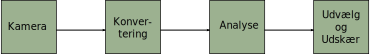
\includegraphics[scale=1]{images/pig-network}
	\caption{Procesnetværk til udskæring af svin på et slagteri.}
	\label{fig:pig-network}
\end{center}
\end{figure}



\subsubsection*{Implementering i Greenletsversionen}
Til at implementere eksemplet uden brug af af RTP-udvidelsen i \pycsp, kan vi oprette hvert svin som et objekt og tilknytte en deadline. Nu kan hver proces evaluere om svinet har overskredet sin deadline, i det tilfælde fjerne svinet, og stoppe den videre behandling. Det er ikke angivet hvordan hele processen startes, men vi antager der findes en form for detektor foran røngtenkameraet, der opfanger når et svin passere og som dermed  starter processen. 
Når detektoren starter hele processen, opretter den svineobjektet som den sender til Røngtenprocessen, samt sender en kopi direkte til udvælgelse og udskæringsprocessen. dermed ved processen at der ankommer et svin som den skal udskære, og hvis den inden deadline får en analyse af svinet, kan den træffe et begrundet valg om hvilken model der skal bruges,  men hvis ikke denne analyse findes, bruges blot standardmodellen. \CRef{fig:pig-network2} viser det endelige  netværk, hvor detektoren er introduceret, og som sender data til hhv. Røntgenprocessen og til Udvælgelse og udskæringsprocessen. 

\begin{figure}
 \begin{center}
  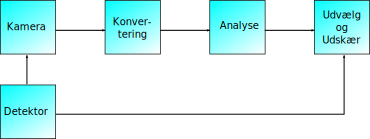
\includegraphics[scale=1]{images/pig-network2}
	\caption{Procesnetværk med detektor til initiering af hvert svin.}
	\label{fig:pig-network2}
\end{center}
\end{figure}

Et problem ved at implementere hele slagterieksemplet i \pycsp er  grænsefladen mellem verden hvor grisene kører på transportbåndet, og  greenletsversionen,  hvor  kun en proces kan være aktiv af gangen. Konvertering og analyse processen arbejder, mens  udskæringsprocessen venter på at svinene kommer inden for rækkevidde. Konvertering- og analysenprocessen  skal dog frivilligt afgive kontrollen, mens svinet er indenfor robottens rækkevidden og hvis de ikke gør, bliver svinet ikke udskåret. I stedet for at det samme system både skal foretage analysen som  styrer robotten, kan vi antage at processerne er mere autonome i deres opbygning. Dette giver at computeren der styrer robotten fungere uafhængigt af de computere der foretager konvertering og analysen. de to computere kan udveksle data igennem f.eks en database, harddisk eller anden delt datastruktur. Hvis analysen bliver færdig gemmes den, i den delte datastruktur, og robotten kan udnytte analysen, Hvis ikke den er klar bruges standard modellen.    



%\subsection{Eksempel 2 - Sensornetværk med høj/lav -prioritet}
%\inline{eks2: skal vise alternation, kan være en sensor som modtager måledata med lav prioritet og som skal sende måledata på opdordring med høj prioritet.}

%\newpage
%\input{../litteratur}
%\newpage
\section{Repræcentation af tid}

I PyCSP foregår kommunikation kun når begge kanalender er klar dvs.
når der findes både en kanalende der vil skrive og en kanalende der vil læse. 
Hvis kun en af kanalenderne er klar, vil den vente indtil
der findes minumum en kanalende af hver type, der er klar. I alternation 
findes muligheden for at tilknytte en timeout til en guard. Dette
giver muligheden for at en process, kun er villig til at vente på at kanalen 
bliver klar inden for en given tidsperiode. 
\begin{lstlisting}[label=Timeout,
  caption=Timeout i Alternation (fra dokumentationen til PyCSP)]
  Alternation([{Timeout(seconds=0.5):None},
               {Cin:None}]).select()
\end{lstlisting} 

I denne alternation er processen villig til at læse fra Cin i 0.5 sekunder. 
Ellers accepteres timeoutguarden og processen er ikke længere villig til at 
læse fra Cin.

Med et simuleringsmiljø er det ikke nok udelukkende kan kunne specifiere en 
timeout på kanalen, det er også nødvændigt at man kan specificere at en proces 
er villig til at kommunikere fra et tidspunkt, samt at den kanalen kun er 
villig til at kommunikere på nuværende tidpunkt, men ikke ud i fremtiden. 

At ville kommunikere fra et given tidspunkt i fremtiden,  svare til at vente 
uden at lave noget indtil det givne tidspunkt for så at forsøge at kommunikere 
fra tidpunktet indtil det kommunktationen lykedes. Dette kan dermed laves helt 
uden en alternation, men ved blot med de to funktioner Wait(time), Cin(). 

At ville være villig til at kommuikere til et given tidspunkt, medfører en ny 
problemstilling, da det introducere muligheden for deadlocks og 
nondeterminisme\fxnote{Er det korrekt?}, for det er ikke defineret hvad tiden 
er hvis det ikke lykkedes at kommunikere i det givne tidsskridt. Der findes to 
muligheder, enten skal scheduleren signalere at der ikke findes mere arbejde 
til dette tidsskridt, og lade processerne fortsætte i samme tidsskridt. 
Alternativt skal tiden tælles op til næste event, hvorefter processerne 
signaleres med at kommunkationen ikke lykkedes. Hvis processerne signalleres 
i samme tidsskridt kan man vælge enten at signallere hver proces en af gangen 
eller samtidigt at signallerer alle processerne. ingen af mulig

processen fortsætte  tildet under antagelsen af problemer.




når tiden er  tidspunkt
til for et findes der allerede \fxnote[inline]{vi skal kunne angive
at vi ønsker at kommunikere men KUN i det tidsskridt vi er i, og at
hvis dette ikke kan lade sig gøre skal vi breake noget alla at have en
timeout på 0} 

%\newpage
%\section{Implementering}

\begin{itemize}
\item DeadlineException
\item Now
\item Release() f.eks i iterationer
\item to køer kaldet has\_priority og no\_priority, og deres brug i funktionen activate
\item Process udvidet med: \\self.inherit\_priotity = []     \\
        self.deadline = None\\
        self.internal\_priority = float("inf")\\
        self.has\_priority = False\\
            if isinstance(arg, pycsp.greenlets.channelend.ChannelEndRead):\\
                arg.channel.\_addReaderProcess(self)\\
            if isinstance(arg, pycsp.greenlets.channelend.ChannelEndWrite):\\
                arg.channel.\_addWriterProcess(self)
\item def Set\_deadline(value,process=None):
\item def Remove\_deadline(process=None):
\item def SetInheritance(process):
\item def ResetInheritance(process):
\item Channel:\\
        self.readerprocesses = []\\
        self.writerprocesses = []

\item Udviddet _read og _write
\item Udvidder match


\end{itemize}


%\input{../test.tex}
\newpage
%\input{../konklusion.tex}

%\input{../jxta-services}
\chapter{Introduktion}
  \section{Problem}
  \section{Kontekst}
  \section{Fremgangsmåde}
  \section{``contributions''}
\chapter{\des}
  \section{Beskrivelse/teori}
    \fxnote[inline]{Beskrivelse af tidsmodellen, teorien omkring den og 
    hvor/hvad den benyttes til. Teori: henvisning til litteratur, bl.a.  
    matematik/beviser for modellen}
  \section{Eksempel}
    \fxnote[inline]{Beskrivelse af eksemplet og hvordan det er relateret til 
    problemet/modellen. Beskrivelse af løsning uden vores tid}
  \section{Design og implementation}
    \fxnote[inline]{Beskrivelse af design med udgangspunkt i eksemplet}
  \section{Evaluering}
    \fxnote[inline]{Evaluering af hvordan eksemplet løses efter den valgte 
    implementation benyttes. Inkluderer test+performance}
  \section{Fremtidigt arbejde}
  \section{Opsummering}
\chapter{Deadline schedulering}
  \section{Beskrivelse/teori}
  \section{Eksempel}
  \section{Design og implementation}
  \section{Evaluering}
  \section{Fremtidigt arbejde}
  \section{Opsummering}
\chapter{Interaktiv tid}
  \section{Beskrivelse/teori}
  \section{Eksempel}
  \section{Design og implementation}
  \section{Evaluering}
  \section{Fremtidigt arbejde}
  \section{Opsummering}
\chapter{Konklusion}
%%%%%%%%%%%%%%%%%%%%%%%%%%%%%%%%%%%%%%%%%%%%%%%%%%%%%%%%%%%%%%%%%%%%%%
%\input{../dibs} / skal det bruges og hvor?

\newpage
\backmatter
%\appendix
%\chapter{Billag}

%\pagenumbering{roman}
%\restorepagenumber

\linespread{1}
\printbibliography

%\chapter{Testresultater}


\section{Testresultater for \des}
\label{app:des-test}
\begin{longtable}{lr}
   	\toprule
    \mc{Test} & \mc{Resultat} \\
    \midrule
    \endfirsthead 
    \toprule
    \mc{Test} & \mc{Resultat} \\
    \midrule
    \endhead % slut efterfølgende headere
    \bottomrule
    \multicolumn{2}{r}{\textit{fortsættes}}
    \endfoot % slut footer
    \bottomrule
    \endlastfoot % slut sidste footer
    Doctest: simulation.Simulation & ok\\
    Doctest: simulation.io & ok\\
    Doctest: guard.testsuite & ok\\
    Doctest: alternation.Alternation & ok\\
    Doctest: alternation.testsuite & ok\\
    Doctest: channel.Channel & ok\\
    Doctest: channel.testsuite & ok\\
    Doctest: process.Parallel & ok\\
    Doctest: process.Spawn & ok\\
    Doctest: process.test\_suite & ok\\
    test\_alternation (test\_simulation.SimulationTestCase) & ok\\
    test\_buffer (test\_simulation.SimulationTestCase) & ok\\
    test\_buffered\_channels (test\_simulation.SimulationTestCase) & ok\\
    test\_decompose (test\_simulation.SimulationTestCase) & ok\\
    test\_io (test\_simulation.SimulationTestCase) & ok\\
    test\_timers1 (test\_simulation.SimulationTestCase) & ok\\
    test\_timers2 (test\_simulation.SimulationTestCase) & ok\\
    test\_timers3 (test\_simulation.SimulationTestCase) & ok\\
    test\_timers\_time\_in\_past (test\_simulation.SimulationTestCase) & ok\\
    test\_wait (test\_io.TestCase) & ok\\
\end{longtable}


\newpage
\section{Testresultater for RTP}
\label{app:rtp-test}
\fxnote{RS: ret stavefejl og sørg for at de to tabeller er formatteret ens}
\begin{longtable}{lr}
   	\toprule
    \mc{Test} & \mc{Resultat} \\
    \midrule
    \endfirsthead 
    \toprule
    \mc{Test} & \mc{Resultat} \\
    \midrule
    \endhead % slut efterfølgende headere
    \bottomrule
    \multicolumn{2}{r}{\textit{fortsættes}}
    \endfoot % slut footer
    \bottomrule
    \endlastfoot % slut sidste footer
test\_Alternation  & ok\\
test\_AlternationChoiseReader  & ok \\
test\_AlternationChoiseWriter  & ok \\
test\_AlternationExecuteReadDeadline  & ok\\
test\_AlternationExecuteSkipDeadline  & ok\\
test\_AlternationExecuteTimeoutDeadline  & ok \\
test\_AlternationExecuteWriteDeadline  & ok \\
test\_Alternationchoise1Deadline  & ok \\
test\_Alternationchoise2Deadline  & ok \\
test\_ChoisemultipleReader  & ok \\
test\_ChoisemultipleReader2  & ok \\
test\_ChoisemultipleWriter  & ok\\
test\_PoisonAndDeadline1  & ok\\
test\_PoisonAndDeadline2  & ok\\
test\_Reader\_Inheritance  & ok\\
test\_RetireAndDeadline  & ok\\
test\_Writer\_Inheritance  & ok\\
test\_channelpriority\_from\_low\_deadline  & ok\\
test\_channelpriority\_from\_low\_deadline2  & ok\\
test\_channelpriority\_from\_no\_deadline  & ok\\
test\_channelpriority\_from\_no\_deadline2  & ok\\
test\_readDeadline  &ok\\
test\_writeDeadline  & ok\\
test\_xreset\_inheritance  & ok\\
test\_xreset\_inheritance\_from\_two\_step  & FAIL\\
\end{longtable}


\fxwarning{inkluder kodeeksempler som best practice}


\chapter{Eksempler}
\section{Best practice for \des}
\lstinputlisting[label=code_wator, caption=WaTor i \code{simulerings}-versionen]{../projects/wator/wator-des.py}
\lstinputlisting[label=code_wator, caption=Simpelt bankeksempel i \code{simulerings}-versionen]{../projects/bank/src/bank03.py}
\lstinputlisting[label=code_wator, caption=Avanceret bankeksempel i \code{simulerings}-versionen]{../projects/bank/src/bank04.py}

\section{Best practice for RTP}  
\lstinputlisting[label=code_wator, caption=Slagterieksemplet \code{RTP}-versionen]{../projects/porks-rtp/porks-rtp.py}
\section{Best practice for IP}  
\lstinputlisting[label=code_wator, caption=Ureksemplet \code{RTP}-versionen]{../projects/watch-ip/watch.py}

 %Fjern %, så vedhæftes bilag (i final)
\end{document}
